\documentclass[a4paper, 11pt]{article}
\usepackage[utf8]{inputenc}
\usepackage[english,russian]{babel}
\usepackage[T1, T2A]{fontenc}
\usepackage{graphicx}
\usepackage{multirow}
\usepackage{pgfplots}
\pgfplotsset{compat=1.9}
\usepackage[left = 2cm, right = 2cm, bottom = 2cm, top = 2cm]{geometry}
\usepackage{listings}
\usepackage{threeparttable}
\usepackage[tableposition=top]{caption}
\usepackage{subcaption}
\DeclareCaptionLabelFormat{gostfigure}{Рисунок #2}
\DeclareCaptionLabelFormat{gosttable}{Таблица #2}
\DeclareCaptionLabelSeparator{gost}{~---~}
\captionsetup{labelsep=gost}
\captionsetup[figure]{labelformat=gostfigure}
\captionsetup[table]{labelformat=gosttable}
\renewcommand{\thesubfigure}{\asbuk{subfigure}}
\captionsetup[table]{labelformat=simple, labelsep = endash, justification = raggedright, singlelinecheck = off}
\usepackage{indentfirst}

\graphicspath{{image/}}

\usepackage[top=2cm, left=2cm, right=2cm, left=2cm]{geometry}
\usepackage{amsmath}

\graphicspath{{image/}}

\newcommand\tline[2]{$\underset{\text{#1}}{\text{\underline{\hspace{#2}}}}$}

\begin{document}
	\begin{titlepage}
		\centering
		{\fontsize{12pt}{5cm}\selectfont \bfseries Министерство образования и науки Российской Федерации} \\ \vspace{0.5cm}
		{\fontsize{7pt}{5cm}\selectfont ФЕДЕРАЛЬНОЕ ГОСУДАРСТВЕННОЕ АВТОНОМНОЕ ОБРАЗОВАТЕЛЬНОЕ УЧРЕЖДЕНИЕ ВЫСШЕГО ПРОФЕССИОНАЛЬНОГО ОБРАЗОВАНИЯ} \\ 
		\vspace{1cm}
		{\fontsize{12pt}{5cm}\selectfont \bfseries САНКТ-ПЕТЕРБУРГСКИЙ УНИВЕРСИТЕТ ИНФОРМАЦИОННЫХ ТЕХНОЛОГИЙ, МЕХАНИКИ И ОПТИКИ} \\ \vspace{1.5cm}

		{\fontsize{14pt}{5cm}\selectfont Кафедра \hspace{1cm} \underline{Систем Управления и Информатики}  \hspace{1cm} Группа \underline{Р3340}} \\ 
		\vspace{2cm}

		{\fontsize{20pt}{5cm}\selectfont \bfseries Лабораторная работа №7} \\
		{\fontsize{20pt}{5cm}\selectfont \bfseries “Анализ точности систем управления”} \\
		{\fontsize{14pt}{5cm}\selectfont Вариант - 25} \\
		\vspace{1.5cm}

		\flushleft

		{Выполнил \hspace{2cm} \tline{(фамилия, и.о.)}{9cm} (подпись)} \\
		\vspace{2cm}

		{Проверил \hspace{2cm} \tline{(фамилия, и.о.)}{9cm} (подпись)} \\
		\vspace{5cm}

		"\underline{\hspace{0.7cm}}"\hspace{0.2cm}\underline{\hspace{2cm}}\hspace{0.2cm}20\underline{\hspace{0.7cm}}г. \hspace{2cm} Санкт-Петербург, \hspace{2cm} 20\underline{\hspace{0.7cm}}г. \\ \vspace{1cm}

		Работа выполнена с оценкой \hspace{1cm} \underline{\hspace{8cm}} \\ 
		\vspace{1cm}
		Дата защиты "\underline{\hspace{0.7cm}}"\hspace{0.2cm}\underline{\hspace{2cm}}\hspace{0.2cm}20\underline{\hspace{0.7cm}}г.

\end{titlepage}


\par
\textbf{Цель работы}
Исследование точностных свойств систем управления.

\begin{center}
\section{Исследование системы с астатизмом нулевого порядка}
\end{center}

\par
Даны передаточная функция объекта управления и характеристики задающего воздействия:
\par
$W(s) = \displaystyle \frac{2}{3s+1}$
\par
$g(t) = 1$
\par
$g(t)=0.5t$
\par
Построим схему моделирования системы с астатизмом нулевого порядка, находящейся в стационарном режиме работы $(g(t) = 1)$, где $H(s)=k$:

\begin{figure}[h!]
\center{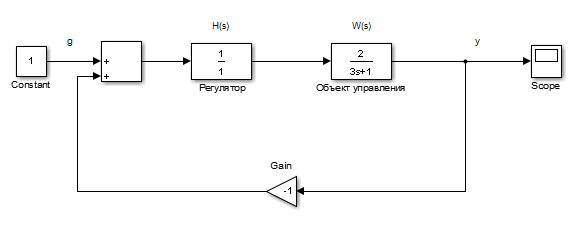
\includegraphics[width=0.75\linewidth]{image/1.png}}
\caption{Схема моделирования системы с астатизмом нулевого порядка с $g(t)=1$}
\label{ris:image}
\end{figure}

\par 
Промоделируем данную систему и получим переходные процессы для $k=1,5,10$:

\begin{figure}[h!]
\center{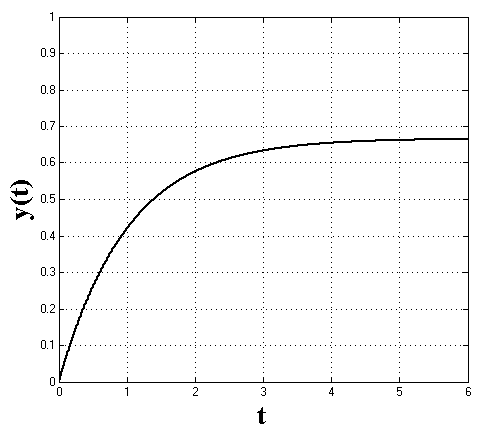
\includegraphics[width=0.75\linewidth]{image/1_2.png}}
\caption{Схема моделирования системы с астатизмом нулевого порядка с $g(t)=1$ и $k=1$}
\label{ris:image}
\end{figure}

\newpage
\begin{figure}[h!]
\center{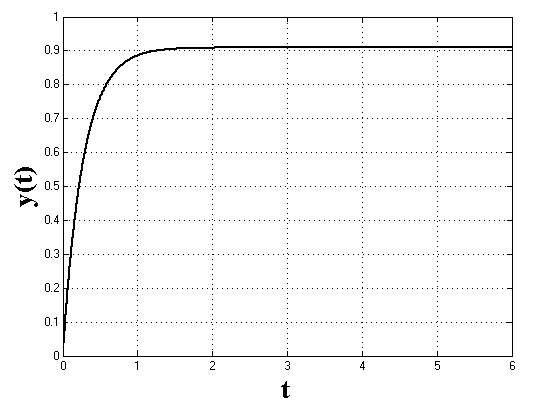
\includegraphics[width=0.75\linewidth]{image/1_3.png}}
\caption{Схема моделирования системы с астатизмом нулевого порядка с $g(t)=1$ и $k=5$}
\label{ris:image}
\end{figure}

\begin{figure}[h!]
\center{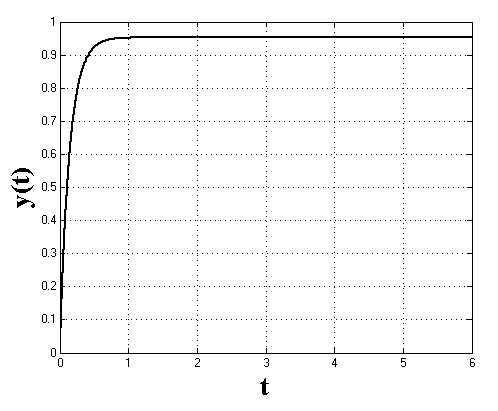
\includegraphics[width=0.75\linewidth]{image/1_4.png}}
\caption{Схема моделирования системы с астатизмом нулевого порядка с $g(t)=1$ и $k=10$}
\label{ris:image}
\end{figure}

\par 
Из графиков переходных процессов определим предельное значение установившейся ошибки $\varepsilon$:
\par 
a) $\varepsilon=0.34$ при $k=1$ 
\par 
b) $\varepsilon=0.09$ при $k=5$
\par 
c) $\varepsilon=0.05$ при $k=10$

\newpage
\par 
Выведем завимость предельного значения установившейся ошибки $\varepsilon$ от $k$. На основе анализа структурной схемы системы можно записать:
\par 
$\displaystyle y=kW(s)e$
\par 
Учитывая, что $y=kW(s)e$
\par 
$\displaystyle e(1+kW(s))=g$
\par 
$e=\displaystyle \frac{g}{1+kW(s)}=\frac{(3s+1)g}{3s+2k+1}$
\par 
В соответствии с теоремой о предельном переходе во временной области, с учётом, что $G(s)=\displaystyle \frac{1}{s}$, имеем:
\par 
$\varepsilon=\lim_{s\to 0}\displaystyle \frac{(3s+1)\frac{1}{s}s}{3s+2k+1}=\frac{1}{2k+1}$
\par 
Выведем экспериментальный и расчётный графики зависимости $\varepsilon(k)$:

\begin{figure}[h!]
\center{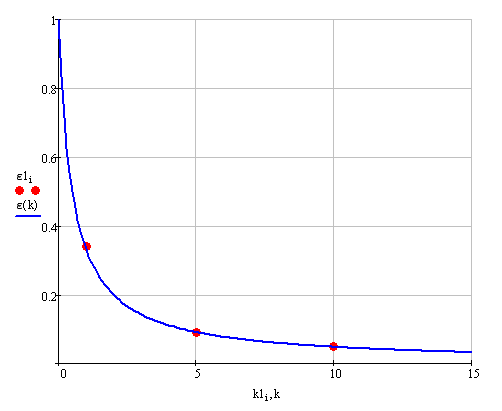
\includegraphics[width=0.75\linewidth]{image/1_5.png}}
\caption{Экспериментальный и расчётный графики зависимости $\varepsilon(k)$}
\label{ris:image}
\end{figure}

\newpage
\par 
Построим схему моделирования системы с астатизмом нулевого порядка, находящейся в режиме движения с постояной скоростью $g(t)=0.5t$, где $H(s)=k$:

\begin{figure}[h!]
\center{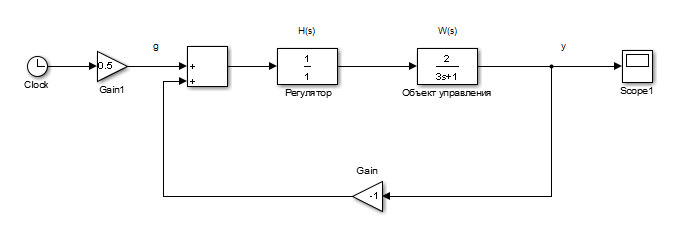
\includegraphics[width=0.75\linewidth]{image/1_6.png}}
\caption{Схема моделирования системы с астатизмом нулевого порядка, движущейся с постоянной скоростью}
\label{ris:image}
\end{figure}

\par 
Промоделируем данную систему и получим переходные процессы для $k=1,5,10$ на интервале времени $t=30c$:

\begin{figure}[h!]
\center{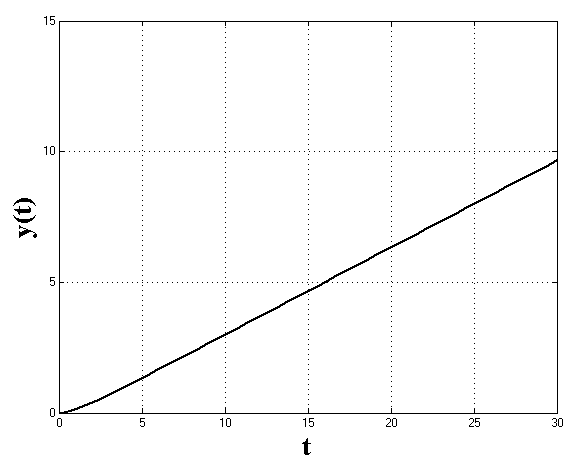
\includegraphics[width=0.75\linewidth]{image/1_7.png}}
\caption{График переходного процесса при $g(t) = 0.5t$ и $k = 1$}
\label{ris:image}
\end{figure}

\newpage
\begin{figure}[h!]
\center{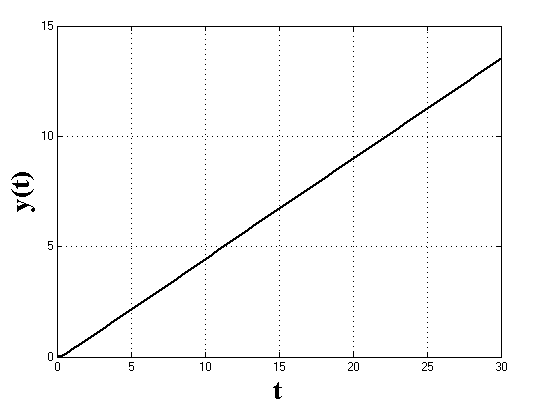
\includegraphics[width=0.75\linewidth]{image/1_8.png}}
\caption{График переходного процесса при $g(t) = 0.5t$ и $k = 5$}
\label{ris:image}
\end{figure}

\begin{figure}[h!]
\center{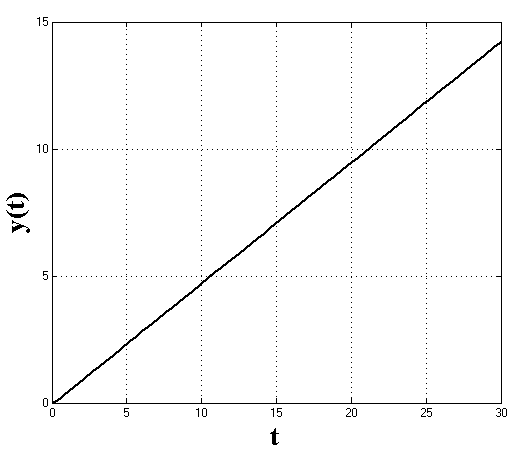
\includegraphics[width=0.75\linewidth]{image/1_9.png}}
\caption{График переходного процесса при $g(t) = 0.5t$ и $k = 10$}
\label{ris:image}
\end{figure}

\newpage
\begin{center}
\section{Исследование системы с астатизмом первого порядка}
\end{center}
\par 
Даны передаточная функция объекта управления и характеристики задающего воздействия:
\par
$W(s) = \displaystyle \frac{2}{3s+1}$
\par
$g(t) = 1$
\par
$g(t)=0.5t$
\par
$g(t)=0.25t^2$

\par 
Построим схему моделирования системы с астатизмом первого порядка, находящейся в стационарном режиме работы $g(t) = 1$, где  $H(s)=\frac{k}{s}$:

\begin{figure}[h!]
\center{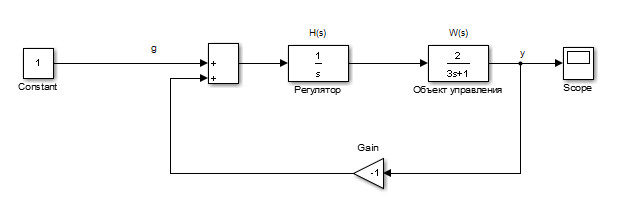
\includegraphics[width=0.75\linewidth]{image/1_10.png}}
\caption{Схема моделирования системы с астатизмом первого порядка, находящейся в стационарном режиме работы}
\label{ris:image}
\end{figure}


\par 
Промоделируем данную систему и получим переходные процессы для $k = 1, 5, 10$:

'\begin{figure}[h!]
\center{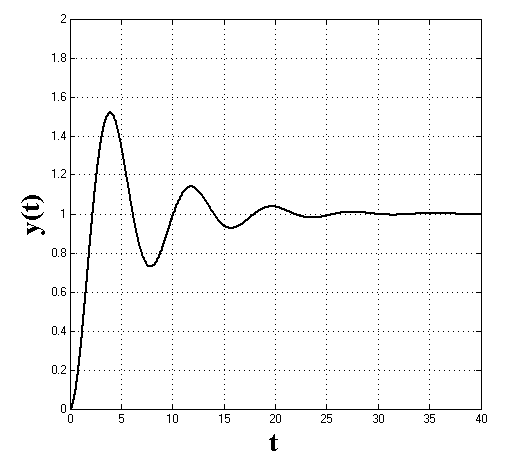
\includegraphics[width=0.75\linewidth]{image/1_11.png}}
\caption{График переходного процесса при $g(t) = 1$ и $k = 1$}
\label{ris:image}
\end{figure}

\newpage
\begin{figure}[h!]
\center{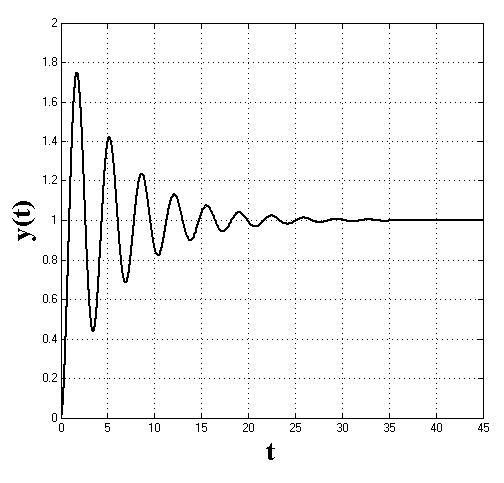
\includegraphics[width=0.75\linewidth]{image/1_12.png}}
\caption{График переходного процесса при $g(t) = 1$ и $k = 5$}
\label{ris:image}
\end{figure}

\begin{figure}[h!]
\center{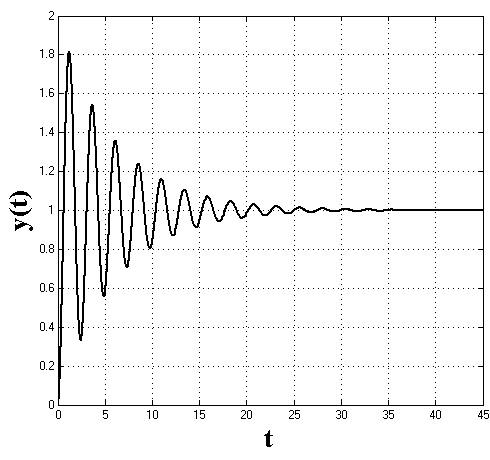
\includegraphics[width=0.7\linewidth]{image/1_13.png}}
\caption{График переходного процесса при $g(t) = 1$ и $k = 10$}
\label{ris:image}
\end{figure}

\newpage
\par 
Из графиков переходных процессов определим предельное значение установившейся ошибки $\varepsilon$:
\par 
$\varepsilon = 0$ при $k = 1$, $k = 5$ и $k = 10$
\par 
Выведем зависимость  предельного значения установившейся ошибки $\varepsilon$ от $k$. На основе анализа структурной схемы системы можно записать:
\par 
$\displaystyle y=W(s)\frac{k}{s}e$
\par 
Учитывая, что $y = g – e$, преобразуем:
\par 
$\displaystyle g-e=W(s)\frac{k}{s}e$
\par 
$\displaystyle e(1+W(s)\frac{k}{s})=g$
\par 
$e=\displaystyle\frac{g}{1+W(s)\frac{k}{s}}=\frac{(3s^2+s)g}{3s^2+s+2k}$
\par 
В соответствии с теоремой о предельном переходе во временной области, с учетом, что $G(s) = 1/s$, имеем: 
\par 
$\varepsilon=\lim_{s\to 0}\displaystyle\frac{(3s^2+s)\frac{1}{s}s}{3s^2+s+2k}=0$
\par 
Выведем экспериментальный и расчетный графики зависимости $\varepsilon(k)$:

\newpage
\begin{figure}[h!]
\center{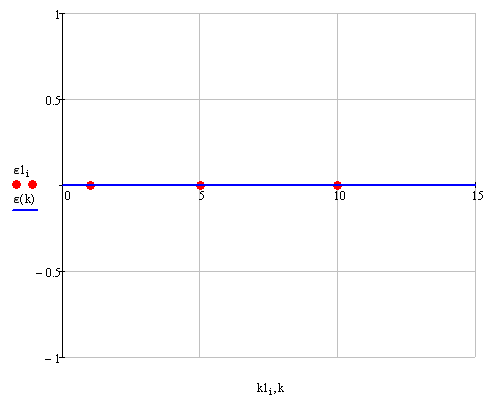
\includegraphics[width=0.75\linewidth]{image/1_14.png}}
\caption{Экспериментальный и расчетный графики зависимости $\varepsilon(k)$:}
\label{ris:image}
\end{figure}

\par 
Построим схему моделирования системы с астатизмом первого порядка, движущейся с постоянной скоростью $g(t) = 0.5t$, где $H(s)=k/s$:

\begin{figure}[h!]
\center{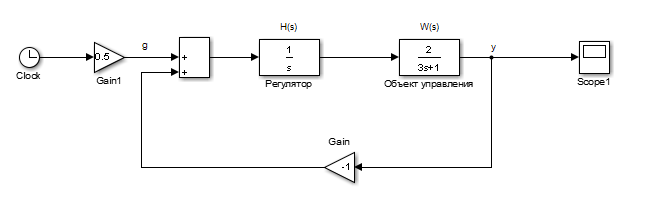
\includegraphics[width=0.75\linewidth]{image/1_15.png}}
\caption{Схема моделирования системы с астатизмом первого порядка, движущейся с постоянной скоростью}
\label{ris:image}
\end{figure}

\par 
Промоделируем данную систему и получим переходные процессы для $k = 1, 5, 10$ на интервале времени $t = 30c$:

\newpage
\begin{figure}[h!]
\center{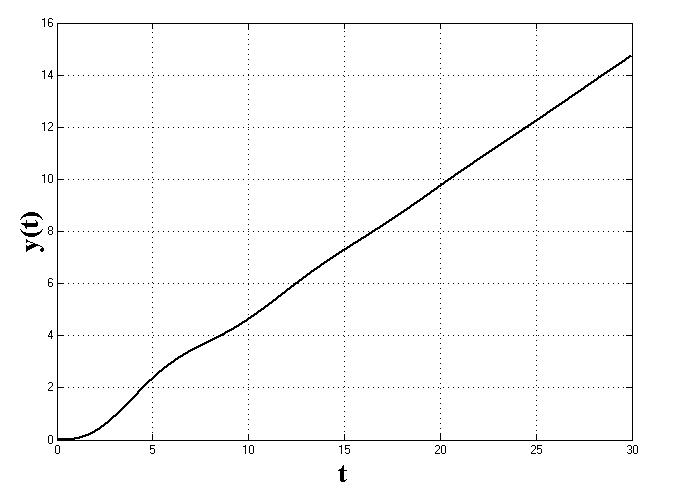
\includegraphics[width=0.75\linewidth]{image/1_16.png}}
\caption{График переходного процесса при $g(t) = 0.5t$ и $k = 1$}
\label{ris:image}
\end{figure}

\begin{figure}[h!]
\center{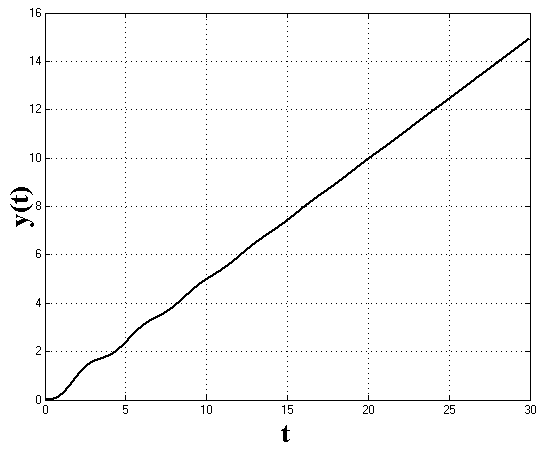
\includegraphics[width=0.75\linewidth]{image/1_17.png}}
\caption{График переходного процесса при $g(t) = 0.5t$ и $k = 5$}
\label{ris:image}
\end{figure}

\newpage
\begin{figure}[h!]
\center{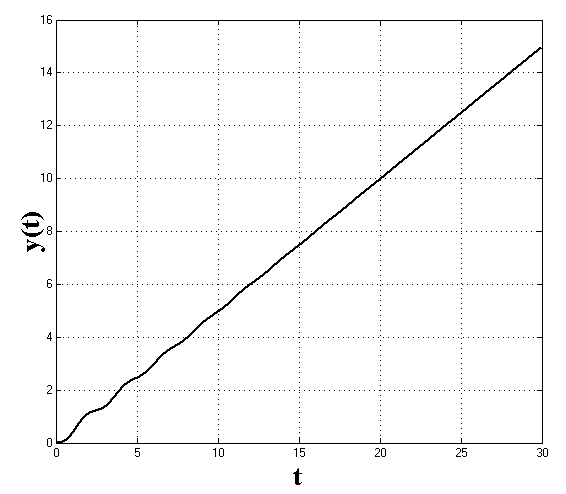
\includegraphics[width=0.75\linewidth]{image/1_18.png}}
\caption{График переходного процесса при $g(t) = 0.5t$ и $k = 10$}
\label{ris:image}
\end{figure}

\par 
Из графиков переходных процессов определим предельное значение установившейся ошибки $\varepsilon$:
\par 
a)	$\varepsilon = 0.24$ при $k = 1$
\par 
b)	$\varepsilon = 0.049$ при $k = 5$
\par 
c)	$\varepsilon = 0.025$ при $k = 10$

\par 
Выведем зависимость  предельного значения установившейся ошибки $\varepsilon$ от $k$. На основе выводов, сделанных  при анализе стационарного режима, получаем:
\par 
$e=\displaystyle\frac{g}{1+W(s)\frac{k}{s}}=\frac{(3s^2+s)g}{3s^2+s+2k}$
\par 
В соответствии с теоремой о предельном переходе во временной области, с учетом, что $G(s) = \frac{0.5}{s^2}$ , имеем:
\par 
$\varepsilon=\lim_{s\to 0}\displaystyle\frac{(3s^2+s)\frac{0.5}{s^2}s}{3s^2+s+2k}=\frac{0.5}{2k}$
\par 
Выведем экспериментальный и расчетный графики зависимости $\varepsilon(k)$:

\newpage
\begin{figure}[h!]
\center{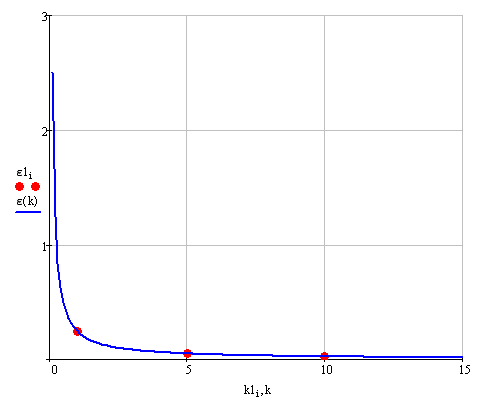
\includegraphics[width=0.75\linewidth]{image/1_19.png}}
\caption{Экспериментальный и расчетный графики зависимости $\varepsilon(k)$}
\label{ris:image}
\end{figure}

\par 
Построим схему моделирования системы с астатизмом первого порядка, движущейся с постоянным ускорением $g(t)=0.25t^2$, где $H(s)=\frac{k}{s}$:

\begin{figure}[h!]
\center{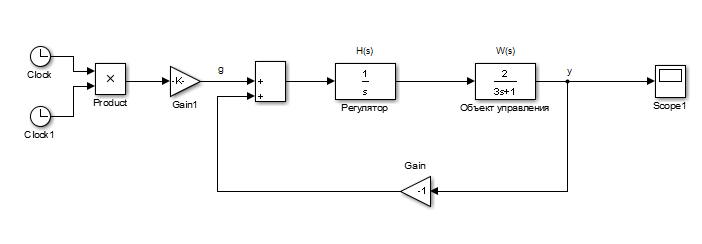
\includegraphics[width=0.75\linewidth]{image/1_20.png}}
\caption{Схема моделирования системы с астатизмом первого порядка, движущейся с постоянным ускорением}
\label{ris:image}
\end{figure}

\par 
Промоделируем данную систему и получим переходные процессы для $k = 1, 5, 10$ на интервале времени $t = 30c$:

\newpage
\begin{figure}[h!]
\center{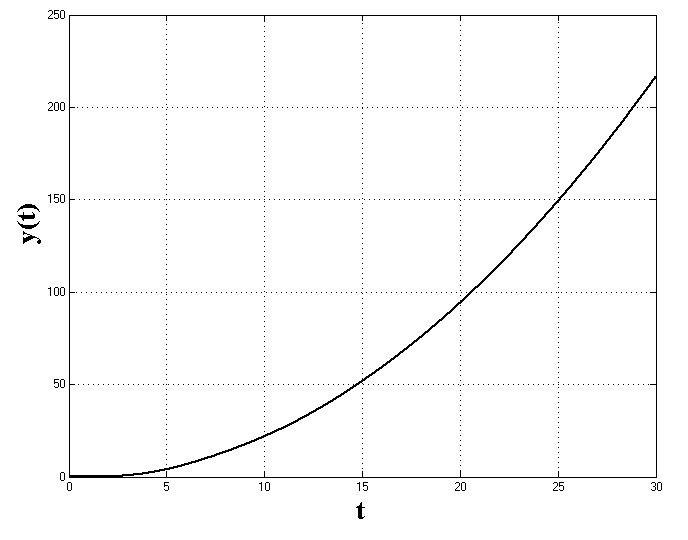
\includegraphics[width=0.75\linewidth]{image/1_21.png}}
\caption{График переходного процесса при $g(t)=0.25t^2$ и $k = 1$}
\label{ris:image}
\end{figure}

\begin{figure}[h!]
\center{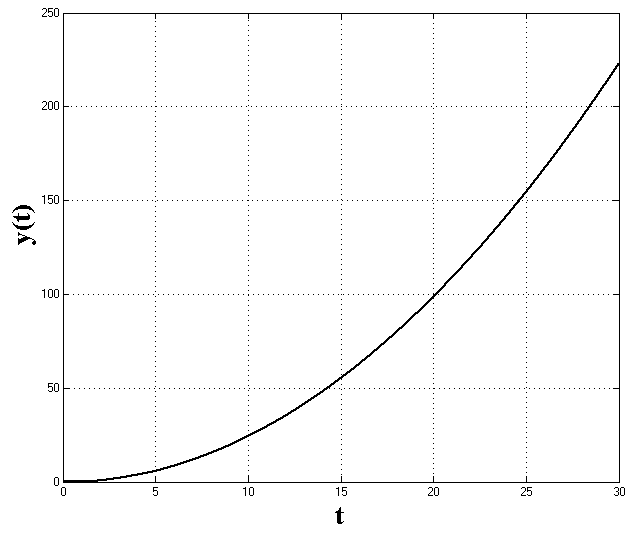
\includegraphics[width=0.75\linewidth]{image/1_22.png}}
\caption{График переходного процесса при $g(t)=0.25t^2$ и $k = 5$}
\label{ris:image}
\end{figure}

\newpage
\begin{figure}[h!]
\center{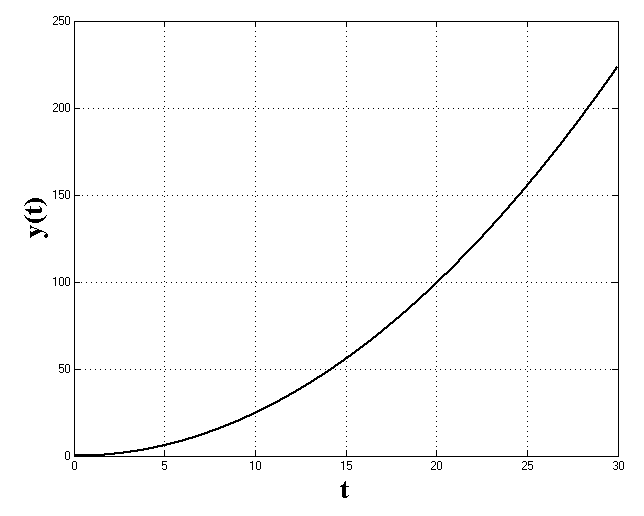
\includegraphics[width=0.75\linewidth]{image/1_23.png}}
\caption{График переходного процесса при $g(t)=0.25t^2$ и $k = 10$}
\label{ris:image}
\end{figure}

\newpage
\begin{center}
\section{Исследование влияний внешних возмущений}
\end{center}
\par 
Построим схему моделирования возмущенной системы со следующими параметрами:
\par 
$W(s)=\displaystyle\frac{2}{(3s+1)}$
\par 
$f_1=1$
\par 
$f_2=-0.5$

\begin{figure}[h!]
\center{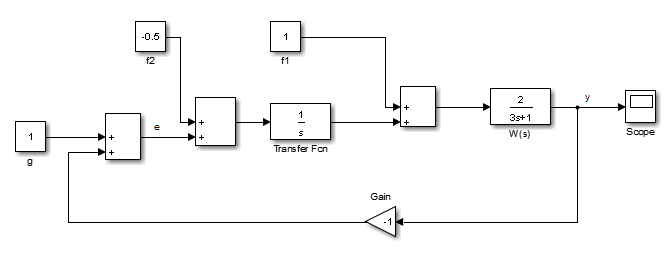
\includegraphics[width=0.75\linewidth]{image/1_24.png}}
\caption{Схема моделирования возмущенной системы}
\label{ris:image}
\end{figure}

\par 
	Промоделируем данную систему, полагая $g(t)=1(t)$  и $f_2=0$, и получим переходный процесс:
	
\begin{figure}[h!]
\center{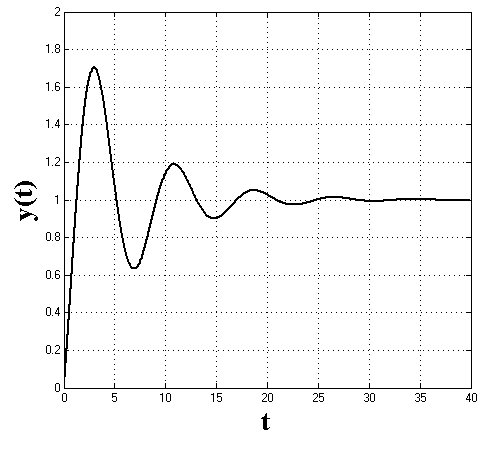
\includegraphics[width=0.75\linewidth]{image/1_25.png}}
\caption{График переходного процесса при $g(t)=1(t)$  и $f_2=0$}
\label{ris:image}
\end{figure}

\par 
Выведем график ошибки слежения:

\newpage
\begin{figure}[h!]
\center{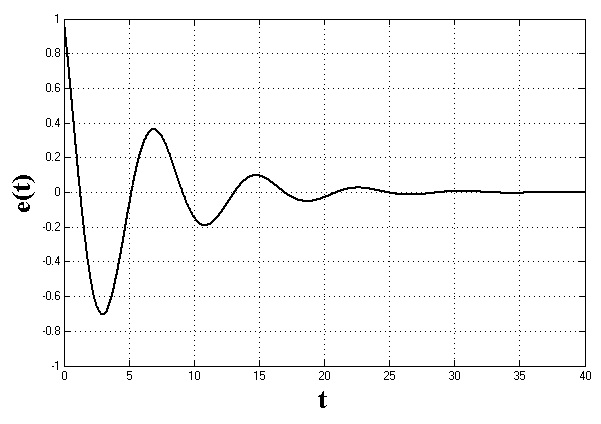
\includegraphics[width=0.75\linewidth]{image/1_26.png}}
\caption{График ошибки слежения $e(t)$ при $g(t)=1(t)$  и $f_2=0$}
\label{ris:image}
\end{figure}

\par 	
Из графика ошибки слежения определяем предельное значение установившейся ошибки: $\varepsilon = 0$ при $g(t)=1(t)$  и $f_2=0$.

\par 
Произведем аналитический расчет установившейся ошибки $\varepsilon$ при $g(t)=1(t)$  и $f_2=0$. На основе анализа структурной схемы системы можно записать:
\par 
$\displaystyle y=W(s)(f_1+\frac{1}{s}e)$
\par 
Выразим $e$, предварительно заменив $y=g-e$:
\par 
$\displaystyle g-e=W(s)(f_1+\frac{1}{s}e)$
\par 
$\displaystyle e(1+W(s)\frac{1}{s})=g-W(s)f_1$
\par 
$e=\displaystyle \frac{g}{1+W(s)\frac{1}{s}}-\frac{W(s)f_1}{1+W(s)\frac{1}{s}}$
\par 
$e=\displaystyle \frac{(3s^2+s)g}{3s^2+s+2}-\frac{2sf_1}{3s^2+s+2}$
\par 
В соответствии с теоремой о предельном переходе во временной области, с учетом, что $G(s) = \frac{1}{s}$, $F1= \frac{1}{s}$ имеем:
\par 
$\varepsilon=\lim_{s\ to 0}\displaystyle\frac{(3s^2+s)\frac{1}{s}s}{3s^2+s+2}-\frac{2s\frac{1}{s}s}{3s^2+s+2}=0$
\par 
Промоделируем данную систему, полагая $g(t)=1(t)$  и $f_1=0$, и получим переходный процесс:

\newpage
\begin{figure}[h!]
\center{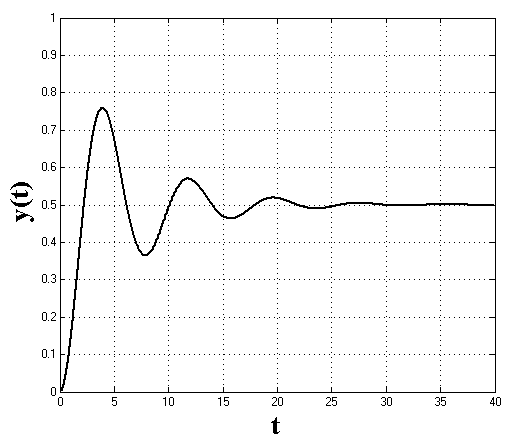
\includegraphics[width=0.75\linewidth]{image/1_27.png}}
\caption{График переходного процесса при $g(t)=1(t)$  и $f_1=0$}
\label{ris:image}
\end{figure}

\par 
Выведем график ошибки слежения:

\begin{figure}[h!]
\center{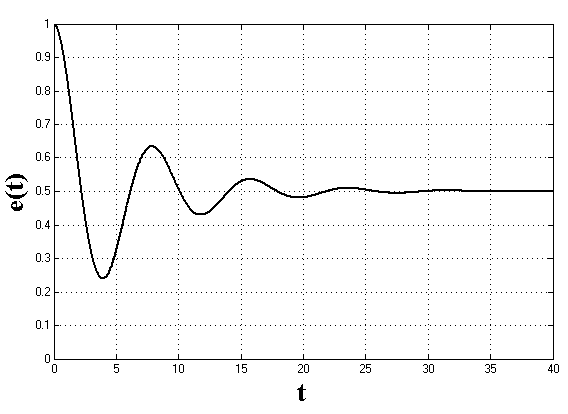
\includegraphics[width=0.75\linewidth]{image/1_28.png}}
\caption{График ошибки слежения $e(t)$  при $g(t)=1(t)$  и $f_1=0$}
\label{ris:image}
\end{figure}

\par 
	Из графика переходного процесса определяем предельное значение установившейся ошибки: $\varepsilon = 0.5$ при $g(t)=1(t)$  и $f_1=0$.
\par 
Произведем аналитический расчет установившейся ошибки $\varepsilon$ при $g(t)=1(t)$  и $f_1=0$. На основе анализа структурной схемы системы можно записать:
\newpage
\par 
$\displaystyle y=W(s)\frac{1}{s}(f_2+e)$
\par 
Выразим $e$, предварительно заменив $y = g – e$:
\par 
$\displaystyle g-e=W(s)\frac{1}{s}f_2$
\par 
$\displaystyle e(W(s)\frac{1}{s}+1)=g-W(s)\frac{1}{s}f_2$
\par 
$e=\displaystyle\frac{g}{W(s)\frac{1}{s}+1}-\frac{W(s)\frac{1}{s}f_2}{W(s)\frac{1}{s}+1}$
\par 
$e=\displaystyle\frac{(3s^2+s)g}{3s^2+s+2}-\frac{2f_2}{3s^2+s+2}$
\par 
	В соответствии с теоремой о предельном переходе во временной области, с учетом, что $\displaystyle G(s) = \frac{1}{s}$, $\displaystyle F1= \frac{-0.5}{s}$ имеем:
\par 
$\varepsilon=\lim_{s\to 0}\displaystyle\frac{(3s^2+s)\frac{1}{s}s}{3s^2+s+2}-\frac{2\frac{-0.5}{s}s}{3s^2+s+2}=0.5$

\newpage
\begin{center}
\section{Исследование установившейся ошибки при произвольном входном воздействии}
\end{center}
\par 
	Построим схему моделирования системы с отрицательной обратной связью со следующими параметрами:
\par 
$\displaystyle W(s)=  \frac{2}{3s+1}$
\par 
$\displaystyle g(t)=2+3sin(0.5t)$
\par 
$H(s)=1$

\begin{figure}[h!]
\center{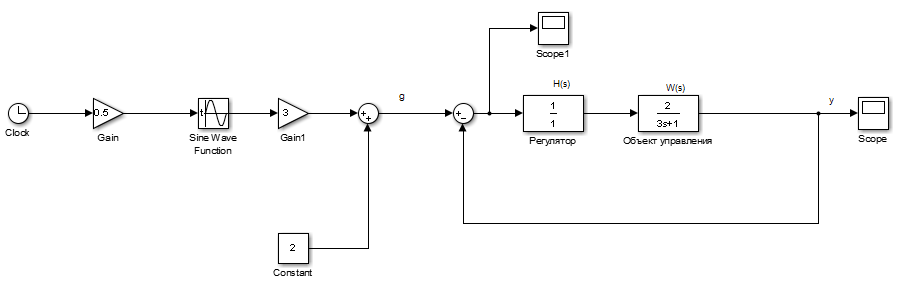
\includegraphics[width=0.75\linewidth]{image/1_29.png}}
\caption{Схема моделирования системы с отрицательной обратной связью}
\label{ris:image}
\end{figure}

\par 
Промоделируем данную систему и получим графики переходного процесса и установившейся ошибки $e_y(t)$:

\begin{figure}[h!]
\center{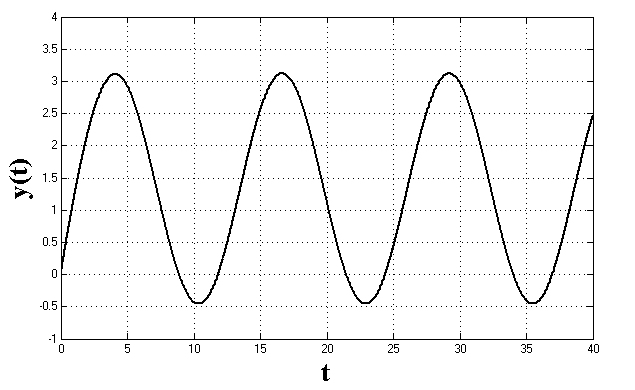
\includegraphics[width=0.75\linewidth]{image/1_30.png}}
\caption{График переходного процесса }
\label{ris:image}
\end{figure}

\newpage
\begin{figure}[h!]
\center{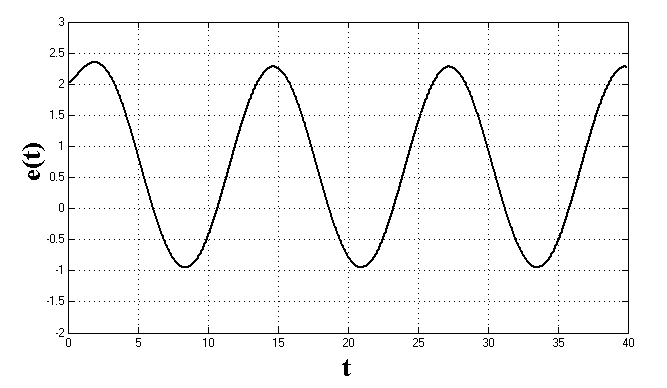
\includegraphics[width=0.75\linewidth]{image/1_31.png}}
\caption{График установившейся ошибки $e_y(t)$}
\label{ris:image}
\end{figure}

\par 
	Получим приближенное аналитическое выражение для $e_y(t)$. Выходная переменная и ошибка связаны следующим выражением:
\par 
$\displaystyle y(t)= W(s)_0e_y(t)$
\par 
$\displaystyle W(s)_0=H(s)W(s)$
\par 
Так как в нашем случае $H(s) = 1$, то:
\par 
$\displaystyle W(s)_0=H(s)W(s)$
\par 
Пользуясь тем, что 
\par 
$\displaystyle e_y(t)=g(t)-y(t)$
\par 
получим:
\par 
$\displaystyle y(t)=W(s)(g(t)-y(t))$
\par 
$y(t)=\displaystyle\frac{W(s)}{1+W(s)}g(t)$
\par 
Обозначим
\par 
$\phi(s)=\displaystyle\frac{W(s)}{1+W(s)}=\frac{2}{3s+1}*\frac{1}{1+\frac{2}{3s+1}}$
\par 
$\phi(s)=\displaystyle\frac{2}{3(s+1)}$
\par 
	Функцию $\phi(s)$ можно разложим в ряд Маклорена, ограничившись первыми тремя членами:
\par 
$\displaystyle \phi(s)=\phi(0)+\phi(0)^{(1)}s+\frac{\phi(0)^{(2)}s^2}{2!}$
\par 
$\displaystyle \phi(0)=c_0=\frac{2}{3}$
\par 
$\phi(0)^{(1)}=c_1=\displaystyle\frac{-2}{3(s+1)^2}=-\frac{2}{3}$
\par 
$\phi(0)^{(2)}=c_2=\displaystyle\frac{4}{3(s+1)^3}=\frac{4}{3}$
\par 
В итоге окончательно получаем:
\par 
$\displaystyle e_y(t)=g(t)-y(t)=g(t)-(\phi(0)+\phi(0)^{(1)}s+\frac{\phi(0)^{(2)}s^2}{2!})g(t)$
\par 
$\displaystyle e_y(t)=(1-\phi(0))g(t)-\phi(0)^{(1)}sg(t)-\frac{\phi(0)^{(2)}s^2}{2!})g(t)$
\par 
Или, переходя к записи через производные:
\par 
$\displaystyle e_y(t)=(1-c_0)g(t)-c_1g(t)^{(1)}-\frac{c_2}{2}g(t)^{(2)}$
\par 
Вычислим производные входного воздействия:
\par 
$\displaystyle g(t)=2+3sin(0.5t)$
\par 
$\displaystyle g(t)^{(1)}=1.5cos(0.5t)$
\par 
$\displaystyle g(t)^{(2)}=-0.75sin(0.5t)$
\par 

\newpage
Получим приближенное аналитическое выражение для $e_y(t)$:
\par 
$\displaystyle e_y(t)\approx\frac{2}{3}+1.5sin(0.5t)+cos(0.5t)$
\par 
Построим по полученному выражению график:

\begin{figure}[h]
\center{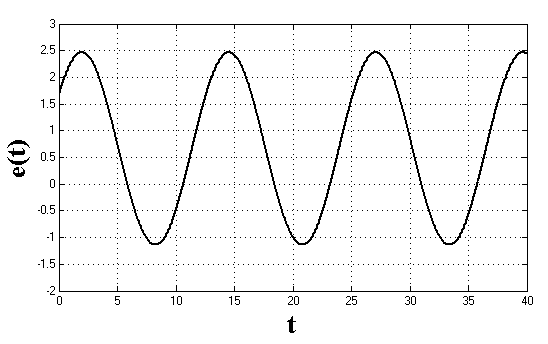
\includegraphics[width=0.75\linewidth]{image/1_32.png}}
\caption{График, построенный на основе приближенного выражения для установившейся ошибки $e_y(t)$}
\label{ris:image}
\end{figure}

\newpage
\begin{center}
\section*{Вывод}
\end{center}
\par 
В ходе проведения данной лабораторной работы были исследованы такие режимы работы систем с астатизмом нулевого и первого порядков, как стационарный, режим движения с постоянной скоростью и режим движения с постоянным ускорением, и построены графики переходных процессов для каждого из режимов. Причем для стационарного режима работы систем с астатизмом нулевого и первого порядков и для режима движения системы первого порядка с постоянной скоростью были получены предельные значения установившейся ошибки $\varepsilon$ при различных значениях параметра $k$ передаточной функции регулятора $H(s)$, а также сделан аналитический вывод зависимости $\varepsilon(k)$ для проверки правильности проведения эксперимента. Проверка показала полное соответствие экспериментальных данных расчетным. Аналогичные выкладки были сделаны и при исследовании возмущенной системы, где также были получены графики переходных процессов и предельные значения установившейся ошибки $\varepsilon$ при различных значениях параметра $k$ передаточной функции регулятора $H(s)$. Аналитический расчет полностью подтверждают данные эксперимента. На последнем этапе данной лабораторной работы было произведено исследование установившейся ошибки $e_y(t)$ при синусоидальном входном воздействии и возможность при аналитическом выводе выражение для $e_y(t)$ ограничиться тремя членами ряда Маклорена. Сравнение графика расчетной $e_y(t)$ с графиком экспериментальной $e_y(t)$ показало, что ограничение возможно с учетом той погрешности, которая возникает при отбрасывании остальных членов. 
\end{document}
